% American Statistical Association style
% Daphne Chan, Ishan Pranav, Ellen Ryoo, Claire Shi

\documentclass[12pt]{article}
\usepackage[english]{babel}
\usepackage{amsmath}
\usepackage{graphicx,psfrag,epsf}
\usepackage{enumerate}
\usepackage{url}
\usepackage{hyperref}
\addtolength{\oddsidemargin}{-.5in}
\addtolength{\evensidemargin}{-.5in}
\addtolength{\textwidth}{1in}
\addtolength{\textheight}{-.4in}
\begin{document}
\def\spacingset#1{\renewcommand{\baselinestretch}
{#1}\small\normalsize} \spacingset{1}
\title{\bf STAT-UB 103 Final Project}
\author{Daphne Chan\\
Ishan Pranav\\
Ellen Ryoo\\
Claire Shi}
\date{April 25, 2023}
\maketitle
\bigskip
\begin{abstract}
Working with real data is the best way to learn statistics. This project is an opportunity to do that.
\end{abstract}
\newpage
\spacingset{1.08}
\section{Introduction}
\subsection{Data sources}
While exploring potential variables to examine, we discovered three data sets available from the Federal Reserve Economic Data website: the Federal Funds Effective Rate (``interest rates''), the unemployment rate among all persons in the United States between 15 and 64 years of age (``unemployment''), and the gross domestic product of the United States (``GDP''). We grouped the data points by quarter and narrowed our focus to the 40 observations between the quarter beginning January 1, 2013, and the quarter beginning October 1, 2022---a 10-year period. 
\begin{itemize}
\item Interest rates: \url{https://fred.stlouisfed.org/series/FEDFUNDS}
\item Unemployment: \url{https://fred.stlouisfed.org/series/LRUN64TTUSQ156S}
\item GDP: \url{https://fred.stlouisfed.org/series/GDP}
\end{itemize}
\subsection{Motivation}
As business students, we are interested in the relationship between macroeconomic measurements because they are the lifeblood of business and are directly linked to the topics we study in our other courses. We hope to discover empirical relationships between the variables that confirm our understanding of economics or reveal insights that our hypotheses overlook. 
\subsection{Hypotheses}
Before exploring the data set, we hypothesize a positive relationship between the interest rate and the GDP. Recalling that during periods of low economic output (low GDP), the Federal Reserve generally implements an expansionary monetary policy, we predict that the interest rate decreases alongside GDP. On the other hand, we expect a negative relationship between the interest rate and unemployment. This is because high unemployment is associated with low economic output, so the Federal Reserve might decrease interest rates to encourage growth.

\section{Scatterplots}
\subsection{Interest rates \emph{vs.} unemployment}
\begin{figure}[ht]
\begin{center}
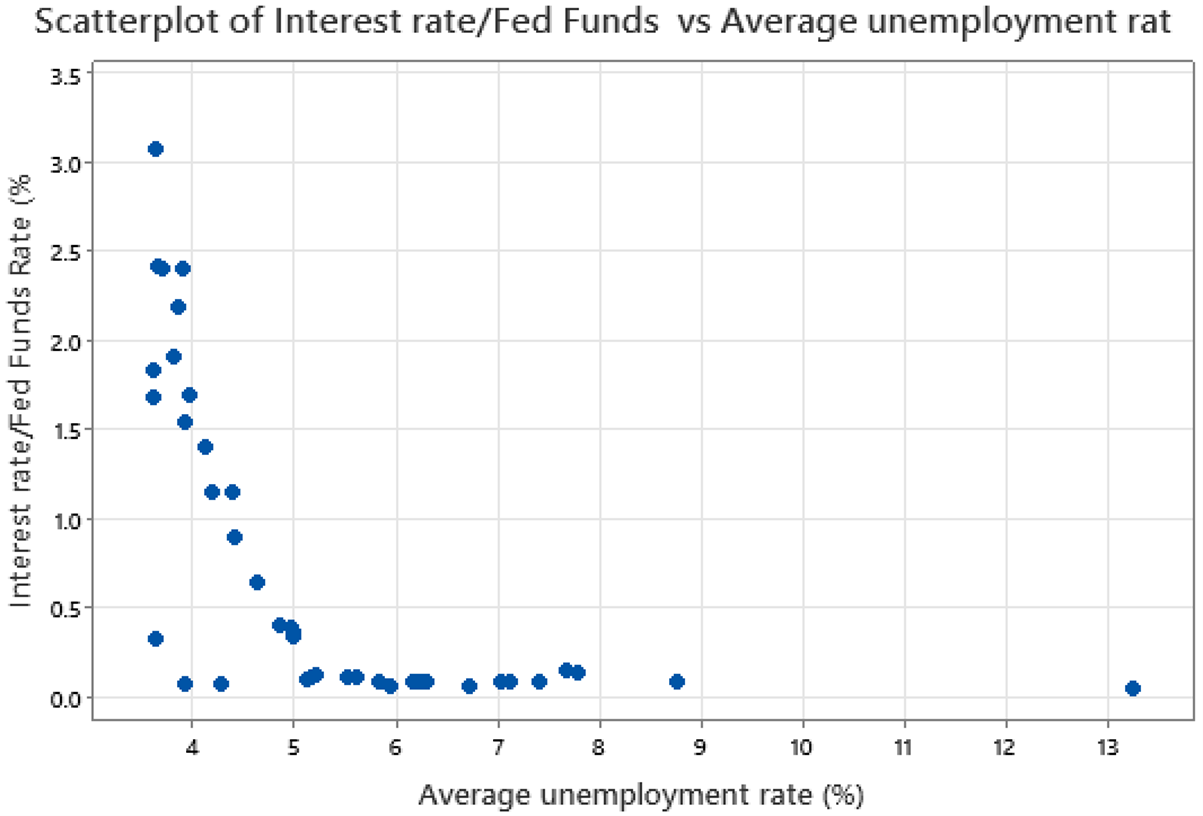
\includegraphics[width=4in]{images/unemployment-scatterplot.png}
\end{center}
\caption{Scatterplot of unemployment (horizontal axis) and interest rates (vertical axis). \label{fig:unemploymentscatterplot}}
\end{figure}
As expected, there is a negative relationship between unemployment and interest rates. The trendline is flat for the portion with high unemployment rates because it is very unusual for interest rates to fall below zero. On the very right, there is one outlier.

There are also three data points significantly below the major trendline. Those observations were collected during the COVID-19 pandemic, which is a potential ``cause'' for the unusual data. Even when the unemployment rate was relatively low, the Federal Reserve was not confident enough in the general economic situation to raise interest rates.
\begin{figure}[ht]
\begin{center}
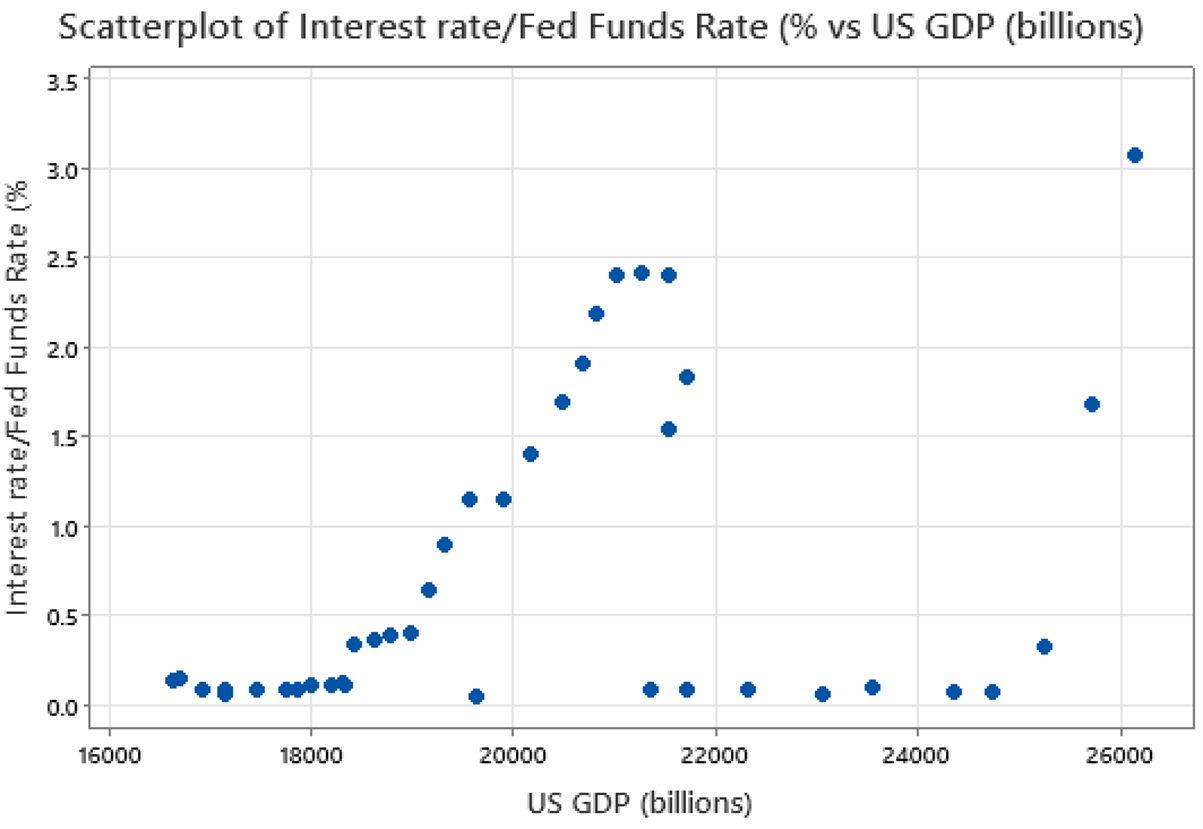
\includegraphics[width=4in]{images/gdp-scatterplot.png}
\end{center}
\caption{Scatterplot of GDP (horizontal axis) and interest rates (vertical axis).
\label{fig:gdpscatterplot}}
\end{figure}
\subsection{Interest rates \emph{vs.} GDP}
The pattern in \autoref{fig:gdpscatterplot} indicates a strong positive correlation up to just under USD\$22,000 billion. The positive correlation falls out of expectations beginning in the last quarter of 2019, then resumes in the second half of 2022.

One potential ``cause'' for the abnormalities is the COVID-19 pandemic, which began at the end of 2019. During the pandemic, GDP dropped drastically from USD\$21,538 billion in the first quarter of 2020 to USD\$19,636 billion in the second quarter of 2020. Although GDP increased from roughly \$20 trillion to \$25 trillion, the interest rate remained near zero because the Federal Reserve was not confident in the nation's economic performance. This is unusual since periods of high output are typically associated with more robust economies. Once the economy stabilized and GDP began to increase steadily, the Federal Reserve increased interest rates to curb inflation. 
\section{Other variables}
This project considers the impact of GDP and unemployment on interest rates. However, other variables may be useful predictors of the interest rate. For example, inflation, consumer spending, investment, government spending, and profits from imports and exports all contribute to this metric. Since the Federal Funds Rate is determined by the Federal Reserve, it is a product of great deliberation and is influenced by many economic indicators that reflect the overall health of the market.
\section{Graphical summaries}
Compared to the scatterplots (\autoref{fig:unemploymentscatterplot} and \autoref{fig:gdpscatterplot}), the graphical summaries (\autoref{fig:interestratesummary}, \autoref{fig:unemploymentsummary}, and \autoref{fig:gdpsummary}) provide insufficient information about outliers. The graphs and boxplots in the graphical summaries only consider one variable at a time. In the case of unemployment, only one outlier meets the ``one-and-a-half-times-the-interquartile-range'' standard for determining an outlier. Meanwhile, the irregularities---like low-interest rates during the high-GDP COVID-19 era---go unnoticed when variables are examined one at a time. For this reason, the scatterplot can provide more insight into whether a specific combination of two variables is unusual.
\begin{figure}[ht]
\begin{center}
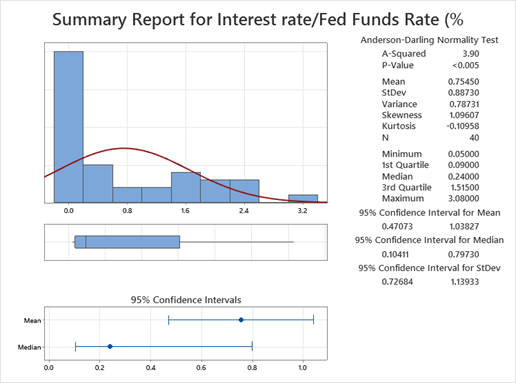
\includegraphics[width=3.5in]{images/interest-rate-summary.png}
\end{center}
\caption{Summary report for interest rates. There are no apparent outliers.\label{fig:interestratesummary}}
\end{figure}
\begin{figure}
\begin{center}
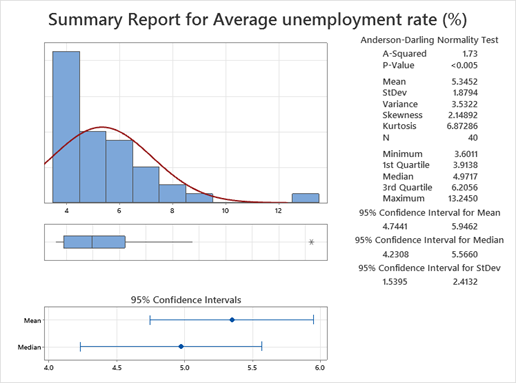
\includegraphics[width=3.5in]{images/unemployment-summary.png}
\end{center}
\caption{Summary report for unemployment. The maximum (13.2 percent) was an outlier in the second quarter of 2020 (represented by a star on the boxplot).\label{fig:unemploymentsummary}}
\end{figure}
\begin{figure}
\begin{center}
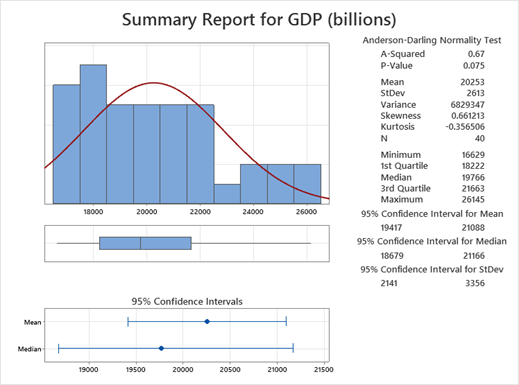
\includegraphics[width=3.5in]{images/gdp-summary.png}
\end{center}
\caption{Summary report for GDP. There are no apparent outliers.\label{fig:gdpsummary}}
\end{figure}
\section{Size-dependent variability}
GDP does not suffer from significant size-dependent variability. The histogram is close to symmetrical; the mean is not significantly larger than the median, relative to the number of data points; the median line on the boxplot is approximately in the middle of the box; and the line on the right of the box is just slightly longer than the line on the left of the box. There are no outliers. Applying a \emph{log}-transformation on the GDP variable does not provide value in statistical analysis.

Meanwhile, the opposite is true for interest rates and unemployment. The histograms for these variables are right-skewed and the boxplots depict the median line on the low (left) side. While there are no outliers for the interest rate variable, the single outlier for the unemployment variable is on the high side (13.2 percent). The interest rate and unemployment variables suffer from size-dependent variability, so applying a \emph{log}-transformation can bring the high outliers in line with the rest of the data and magnify the lower observations, allowing clearer analysis of the data. 
\begin{figure}[ht]
\begin{center}
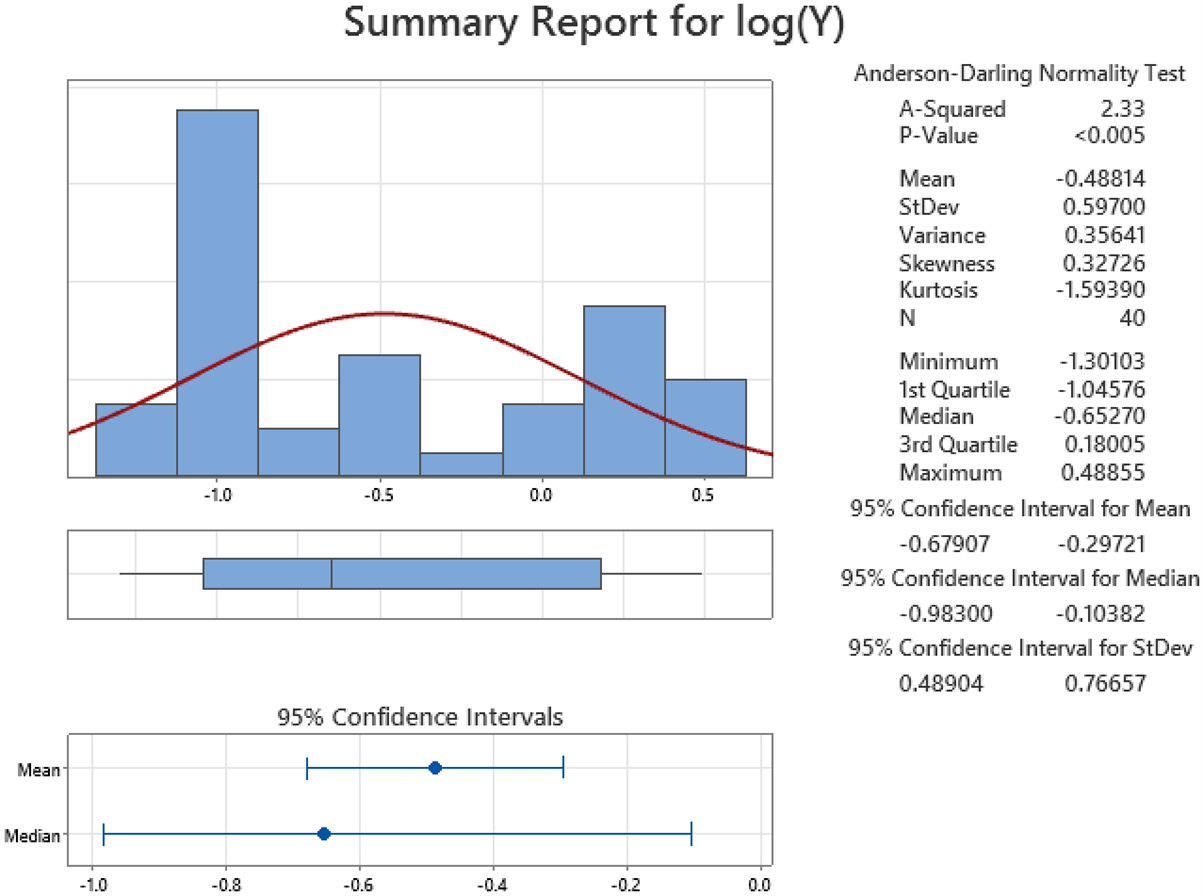
\includegraphics[width=4in]{images/log-interest-rate-summary.png}
\end{center}
\caption{Summary report for interest rates after applying a \emph{log}-transformation. There are no apparent outliers.\label{fig:loginterestratesummary}}
\end{figure}
\begin{figure}[ht]
\begin{center}
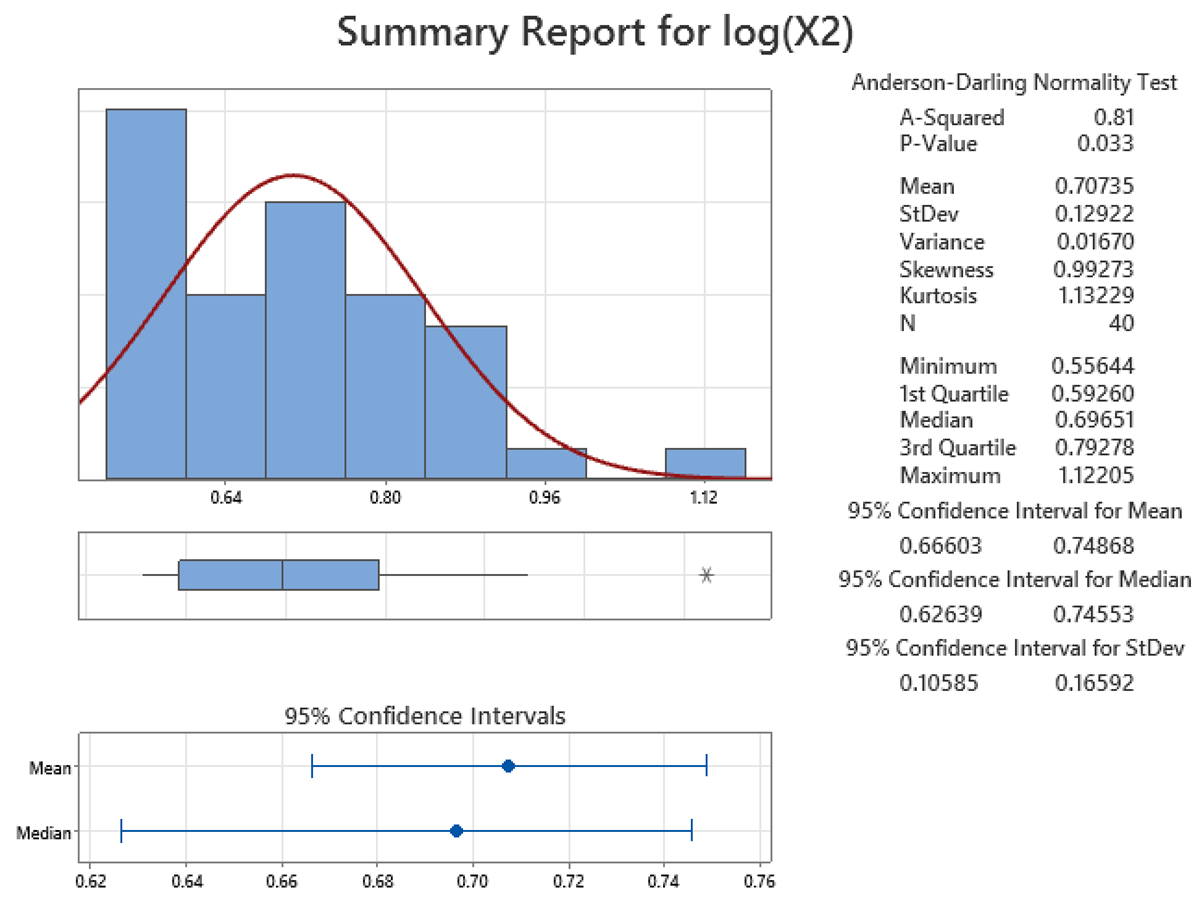
\includegraphics[width=4in]{images/log-unemployment-summary.png}
\end{center}
\caption{Summary report for unemployment after applying a \emph{log}-transformation. The outlier of 13.2 percent remains apparent.\label{fig:logunemploymentsummary}}
\end{figure}
\section{Logarithmic-scale scatterplots}
\begin{figure}[p]
\begin{center}
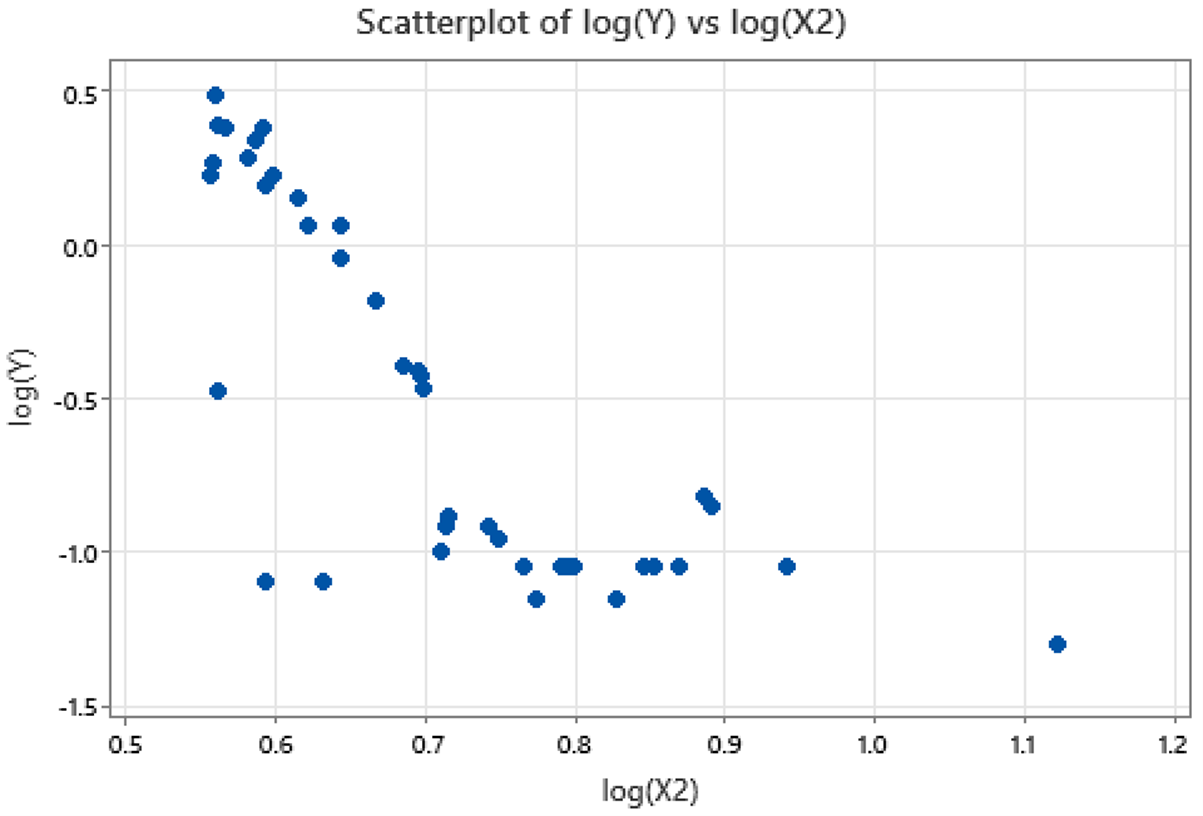
\includegraphics[width=3.5in]{images/log-unemployment-log-scatterplot.png}
\end{center}
\caption{Scatterplot of unemployment (horizontal axis, logarithmic) and interest rates (vertical axis, logarithmic).\label{fig:logunemploymentlogscatterplot}}
\end{figure}
\begin{figure}[p]
\begin{center}
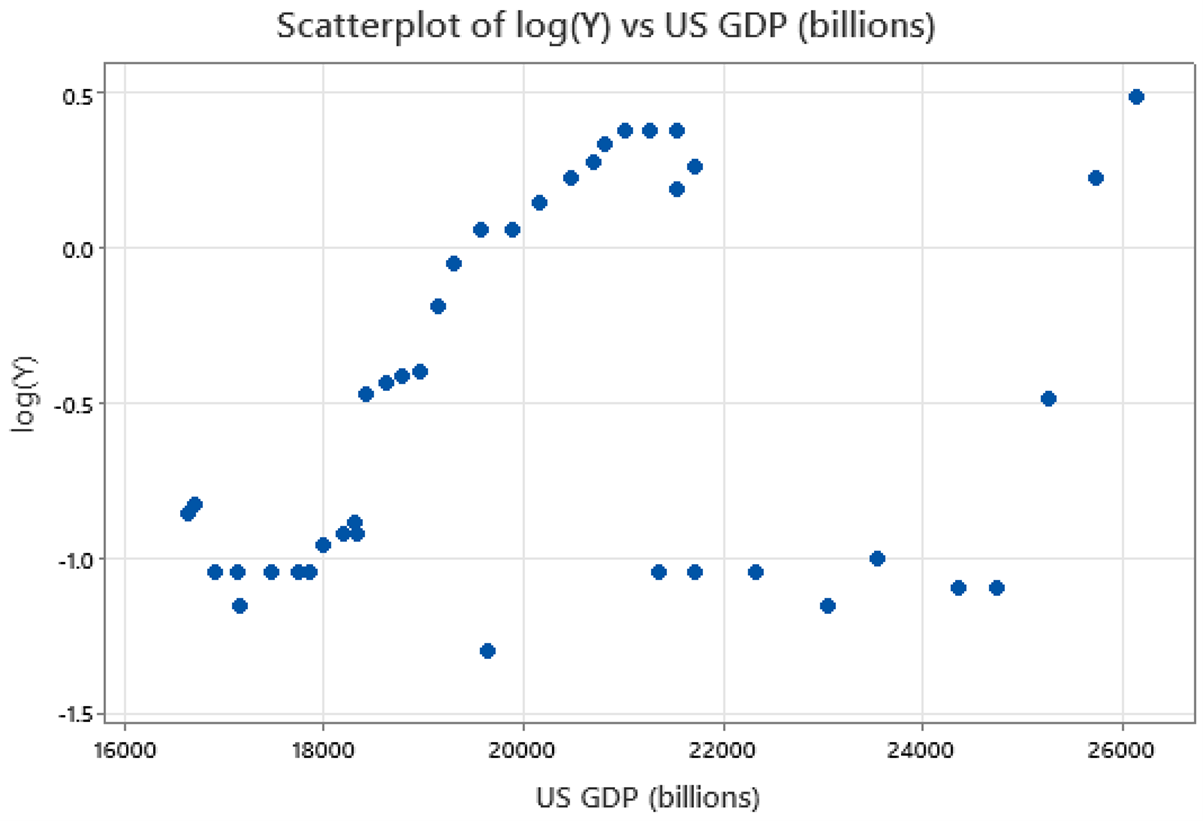
\includegraphics[width=3.5in]{images/gdp-log-scatterplot.png}
\end{center}
\caption{Scatterplot of GDP (horizontal axis) and interest rates (vertical axis, logarithmic).\label{fig:gdplogscatterplot}}
\end{figure}
\subsection{Results of \emph{log}-transformation and conclusion}
As depicted in \autoref{fig:logunemploymentlogscatterplot} and \autoref{fig:gdplogscatterplot} below, taking the natural logarithm of the interest rate and unemployment observations yields a clearer negative relationship between unemployment and interest rates and a clearer positive relationship between GDP and interest rates. The correlation is quite strong in both cases.

Having analyzed the data we confirmed our hypothesis: there is a strong positive relationship between GDP and interest rates and a strong negative relationship between unemployment and interest rates.

We conclude that there exists a positive correlation between economic output (as measured by GDP) and the logarithm of the interest rate and a negative correlation between the logarithm of the unemployment rate and the logarithm of the interest rate.

\section{Anderson--Darling test}
\subsection{Gaussian probability plot}
\begin{figure}[h]
\begin{center}
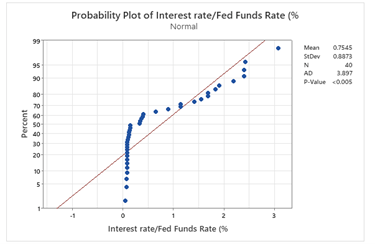
\includegraphics[width=4in]{images/interest-rate-probability-plot.png}
\end{center}
\caption{Normal probability plot for interest rates. \label{fig:interestrateprobabilityplot}}
\end{figure}
The pattern in the plot of interest rates (\autoref{fig:interestrateprobabilityplot}) seems to indicate non-normality, as the data do not fall in a straight line. In particular, the points on the left end bend vertically below the line which indicates that the left tail is longer than that of a normal distribution. The points on the right end stray away from the line before bending back up.
\subsection{\textit{P}-value}
The $P$-value resulting from the Anderson--Darling test seems to indicate non-normality since the value is less than 0.005. In the Anderson--Darling hypothesis test, the null hypothesis is that the data follows a Gaussian (normal) distribution, and the alternative hypothesis is that the data do not follow a normal distribution. A low $P$-value indicates that the test statistic obtained is very unlikely given that the null hypothesis. Using a significance level of five percent ($\alpha$=0.05), there is convincing evidence to reject the null hypothesis: The $P$-value is far smaller than 5 percent. Therefore, we conclude that interest rates are not normally distributed.
\subsection{Comparison with summary report}
The normal curve depicted on the summary report for the interest rate (\autoref{fig:interestratesummary}) is heavily skewed to the right. This finding aligns with the descriptive statistics: We see a large portion of the data accumulated between 0.0 and 0.5. As the interest rate increases, there are fewer and fewer points included within the range, providing a skewed distribution.
\section{Anderson--Darling test after logarithmic scaling}
\subsection{Normal probability plot}
\begin{figure}[h]
\begin{center}
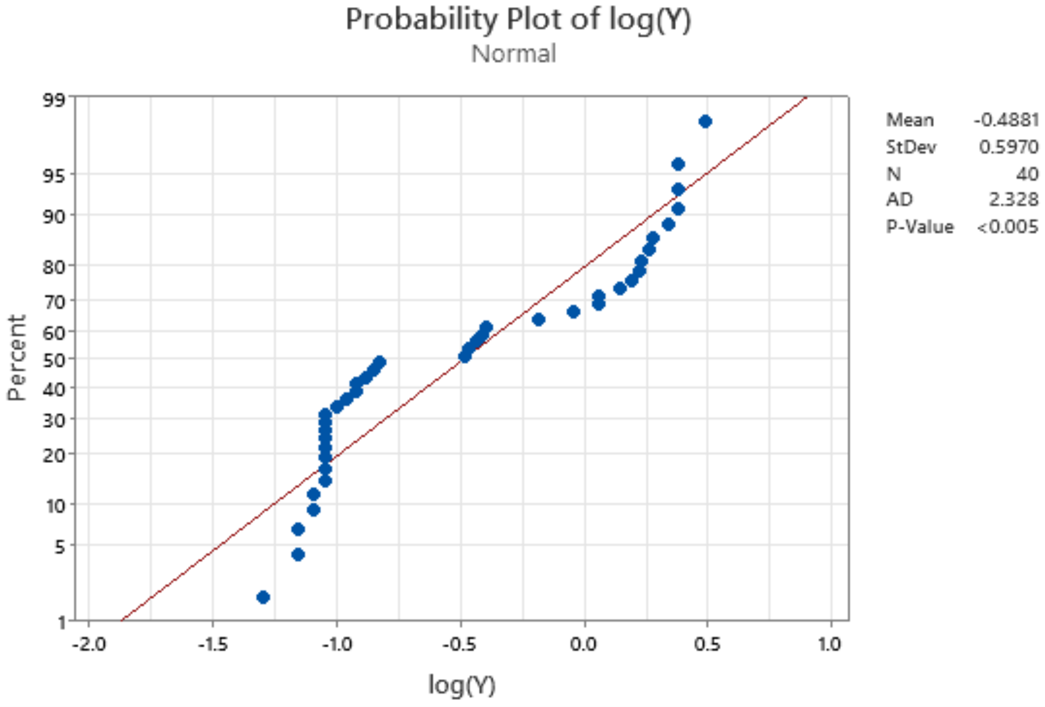
\includegraphics[width=4in]{images/log-interest-rate-probability-plot.png}
\end{center}
\caption{Gaussian probability plot for the logarithm of the interest rate. \label{fig:loginterestrateprobabilityplot}}
\end{figure}
The pattern in the plot of \textit{log}-scaled interest rates (\autoref{fig:loginterestrateprobabilityplot}) seems to indicate non-normality because the points do not form a straight line. Instead, they bend downwards on the left side of the plot, which means that the lower tail is longer.
\subsection{\textit{P}-value}
The $P$-value resulting from the Anderson--Darling test also indicates non-normality because it is very close to zero. There is convincing evidence at the $\alpha=0.05$ significance level to reject the null hypothesis. Therefore, we conclude that the logarithm of the interest rate is not normally distributed.
\subsection{Comparison with summary report}
Once again, the findings based on the plot and the Anderson--Darling test align with the summary report for the logarithm of the interest rate in \autoref{fig:loginterestratesummary}. After applying a \textit{log}-transformation, the distribution now fits the regression line slightly better. According to the descriptive statistics, there is still a large portion of the data accumulated near $-1.0$ and 0.3, but applying the \textit{log}-transformation has resulted in less skew.
\section{Simple linear regression}
\section{Multiple linear regression}
\section{Comparison of regression methods}
\section{Cook's distance}
\section{Residual analysis}
\section{Akaike information criterion, corrected (AICc)}
\end{document}
